% !TEX root = main.tex
% -*- coding: utf-8 -*-
% \LoadClass[12pt]{extarticle}
\documentclass[UTF8,a4paper,12pt]{ctexart}

% Configuration des packages et paramètres pour le document
\RequirePackage[french]{babel}
\RequirePackage[T1]{fontenc}
\RequirePackage{graphicx}
\RequirePackage{xcolor}
\RequirePackage[a4paper, left=2.5cm, right=2cm, top=2cm, bottom=2cm]{geometry}
\RequirePackage{multicol}
\RequirePackage{fancyhdr}
\RequirePackage{ifthen}
\setlength{\headheight}{14.5pt}
\addtolength{\topmargin}{-2.5pt}
\RequirePackage{lipsum}
\RequirePackage{float}
\RequirePackage{subfigure}
\RequirePackage{hyperref}
\hypersetup{colorlinks=true,linkcolor=black}
\graphicspath{ {./images/} }

% Customization for headings and sections
\renewcommand{\headrulewidth}{0.4pt}
\renewcommand{\footrulewidth}{0.4pt}
\renewcommand{\thesection}{\Roman{section}}
\renewcommand{\refname}{Bibliographie}

% Définition des styles de titres
\RequirePackage{titlesec}
\titleformat{\section}
  {\normalfont\fontsize{22}{26}\bfseries}{\thesection}{1em}{}
\titleformat{\subsection}
  {\normalfont\fontsize{14}{17}\bfseries}{\thesubsection}{1em}{}
\titleformat{\subsubsection}
  {\normalfont\fontsize{12}{14}\bfseries\itshape}{\thesubsubsection}{1em}{}

% Définition des marges pour les paragraphes
\setlength{\parindent}{1.5cm} % Indentation for new paragraphs
\setlength{\parskip}{1ex} % Spacing between paragraphs

% Configuration des en-têtes et pieds de page
\pagestyle{fancy}
\fancyhf{}
\fancyhead[C]{\MyHeader}

\fancyfoot{}
\fancyfoot[R]{\thepage}

\fancyfoot[C]{
    \textit{\MyFooter}\par
    {\color{red}\textit{
        Rapport 
        \ifthenelse{\boolean{confidential}}{confidentiel}{non confidentiel et
        \ifthenelse{\boolean{onlinePublish}}{publiable}{non publiable}
        sur internet}}
        }
}

% ==========================================================
% Les définitions ci-dessous ne doivent pas être modifiées
% ==========================================================

\def\MyHeader{\title}
\def\MyFooter{\authorName / \hostName}
\newboolean{confidential}
\newboolean{onlinePublish}
\def\documentTitle{Projet de Recherche (PRe)} % Titre du document
\def\enstaLogo{ensta.jpg} % Logo de l'école

% ==========================================================

% ==========================================================
% Les définitions ci-dessous doivent être personnalisées 
% en fonction des détails spécifiques.
% ==========================================================

\def\hostLogo{ensta.jpg} % Logo de l'organisme d'accueil
\def\speciality{Informatique} % Spécialité
\def\academicYear{2023-2024} % Année académique
\def\title{Application de l'IA à l'analyse des données} % Titre du rapport de stage
\def\authorName{Jean Dupont} % Nom de l'auteur
\def\schoolTutor{Pierre Martin} % Nom du tuteur ENSTA Paris
\def\classPromotion{2026} % Promotion
\def\hostTutor{Lucie Lefevre} % Nom du tuteur de l'organisme d'accueil
\def\internshipDuration{Stage éffectué du 01/06/2023 au 31/08/2023} % Durée du stage
\def\hostName{Institut de Recherche en Informatique} % Nom de l'organisme d'accueil
\def\hostAddress{123 rue de la Science, 75000 Paris - France} % Adresse de l'organisme d'accueil

\setboolean{confidential}{false} % Confidentialité du rapport
\setboolean{onlinePublish}{true} % Publication en ligne autorisée

% ==========================================================

\begin{document}
%------------------------Page de titre------------------------%
\thispagestyle{empty} % Pas de numéro de page
\hspace*{-1.5cm}\includegraphics[height=4cm]\enstaLogo
\hfill
\includegraphics[height=4cm]\hostLogo
\par
% \vspace{0.5cm}
\centering % Everything on this page will be centered
    
\vspace*{\fill} % Vertically center the page contents
    
\textbf{\Huge \documentTitle}\par
\vspace{0.5cm}
\textbf{\Large Spécialité : \speciality}\par
% \vspace{0.5cm}
\textbf{\Large Année scolaire : \academicYear}\par
\vspace{1.0cm}
{\Huge\bfseries \title}\par
% \vspace{1cm}

\includegraphics[height=4cm]{illustration.png} % Illustration facultative
\vspace{1cm}
\fcolorbox{red}{white}{\parbox{0.8\linewidth} {
    \centering
    \vspace{0.3cm}
    \color{red}\textbf{\Large Mention de confidentialité}\par
    \vspace{0.3cm}
    \textbf{ 
        \ifthenelse{\boolean{confidential}}{le document est confidentiel}{le document est non confidentiel\ifthenelse{\boolean{onlinePublish}}{. Il peut donc être consultable en ligne par tous.}{ et consultable au format électronique uniquement sur place à la bibliothèque de l'ENSTA Paris.}}
    }
    \vspace{0.3cm}
    }
}
    
% \vspace{1cm}
\begin{multicols}{2}
    \textbf{\small Auteur :\authorName}\par
    \textbf{\small Tuteur ENSTA Paris : \schoolTutor}\par
    \columnbreak
    \textbf{\small Promotion: \classPromotion}\par
    \textbf{\small Tuteur organisme d'accueil : \hostTutor}\par
\end{multicols}
\par\vspace{1cm}
\textbf{\large\internshipDuration}\par\vspace{1cm}
{\raggedleft
    \textbf{NOM de l'organisme d'accueil : \hostName}\par
    \textbf{Adresse : \hostAddress}\par
}
    
\vspace*{\fill} % Vertically center the page contents
%-------------------------------------------------------------%

%----------------------Page de garde vierge----------------------%
\newpage % Insère une page totalement vide
~\newpage
%-------------------------------------------------------------%
\raggedright
%----------------------Page de titre----------------------%
\section*{Résumé}
\addcontentsline{toc}{section}{Résumé}

\hspace{8mm} Texte texte texte texte texte texte texte texte texte texte texte texte. Texte texte texte texte texte texte texte texte texte texte texte texte texte. Texte texte texte texte texte texte texte texte texte texte texte texte texte Texte texte texte texte texte texte texte texte texte texte texte texte texte texte. Texte texte texte texte texte texte texte texte texte texte texte texte texte texte. Texte texte texte texte texte texte texte texte texte texte texte texte texte.

\hspace{8mm} Texte texte texte texte texte texte texte texte texte texte texte texte texte texte. Texte texte texte texte texte texte texte texte texte texte texte texte texte texte.

\vspace{0.3cm}
\textbf{\underline{Mots-clés: }}

keyword1, keyword2, keyword3

\vfill

\section*{Abstract}

\hspace{8mm} Texte texte texte texte texte texte texte texte texte texte texte texte. Texte texte texte texte texte texte texte texte texte texte texte texte texte. Texte texte texte texte texte texte texte texte texte texte texte texte texte Texte texte texte texte texte texte texte texte texte texte texte texte texte texte. Texte texte texte texte texte texte texte texte texte texte texte texte texte texte. Texte texte texte texte texte texte texte texte texte texte texte texte texte.

\hspace{8mm} Texte texte texte texte texte texte texte texte texte texte texte texte texte texte. Texte texte texte texte texte texte texte texte texte texte texte texte texte texte.

\vspace{0.3cm}
\textbf{\underline{Keywords: }}

keyword1, keyword2, keyword3

\vfill

\newpage
%-------------------------------------------------------------%

%----------------------Des remerciements----------------------%
~\newpage
\section*{Remerciements}
\addcontentsline{toc}{section}{Remerciements}
\lipsum[1]
\newpage
%-------------------------------------------------------------%

%----------------------Table des matières----------------------%
% Table des matières
\raggedright
\renewcommand{\contentsname}{\hfill\bfseries\Large Table des matières\hfill}

\addcontentsline{toc}{section}{Table des matières}
{\tableofcontents
\thispagestyle{fancy}
}
\newpage
%-------------------------------------------------------------%

%----------------------Table des figures----------------------%
% Table des figures
\renewcommand{\listfigurename}{\hfill\bfseries\Large Table des illustrations\hfill}
\addcontentsline{toc}{section}{Table des illustrations}
\listoffigures
\newpage
%-------------------------------------------------------------%



%----------------------Corps du rapport----------------------%
\section{Section}
\lipsum[6]\cite{dupont2023}
\subsection{Subsection}
\lipsum[8] Voir Figure \ref{Fig1}.

\begin{figure}[h]
\centering
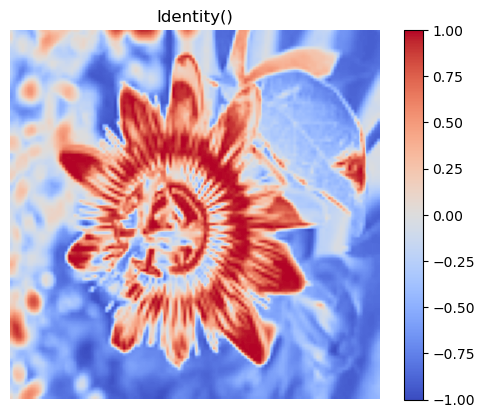
\includegraphics[width=0.7\textwidth]{figure1.png}
\caption{Exemple Figure}
\label{Fig1}
\end{figure}

\subsubsection{Subsubsection}
\lipsum[9]

\newpage
\bibliographystyle{plain} % Style de la bibliographie
\bibliography{ref.bib} % Fichier de références bibliographiques
\addcontentsline{toc}{section}{Bibliographie}

\newpage
\appendix
\section{Annexes 1}
\lipsum[2]
\subsection{sub}
\lipsum[1]

\end{document}
